\documentclass[aspectratio=1610]{beamer}

\usetheme{KTH}

% remove this if using XeLaTeX or LuaLaTeX
\usepackage[utf8]{inputenc}
\usepackage{graphics}
\usepackage{caption}
\usepackage{subcaption}
\usepackage{csquotes} % Recommended by biblatex
\usepackage{biblatex}

\DeclareRobustCommand{\bbone}{\text{\usefont{U}{bbold}{m}{n}1}}

\DeclareMathOperator{\EX}{\mathbb{E}}
\DeclareMathOperator{\Lagr}{\mathcal{L}}

\addbibresource{ex.bib}

\begin{document}

%%%%%%%%%%%%%%%%%%%%%%%%%%%%%%%%%%%%%%%%%%%%%%%%%%%%%%%%%%%%
\begin{frame}

  \vspace{0.02\textheight}
  
  \begin{Large}
    Investigation of deep learning approaches for overhead imagery analysis 
  \end{Large}

  \vspace{0.1\textheight}

  \begin{small}
    \textit{Joar Gruneau}
  \end{small}
\end{frame}


%%%%%%%%%%%%%%%%%%%%%%%%%%%%%%%%%%%%%%%%%%%%%%%%%%%%%%%%%%%%

\usebackgroundtemplate{\vbox{\null\vspace{3mm}
  \hspace{3mm}\pgfuseimage{kthlogosmall}\par
  \vspace{72mm}\hbox{\hspace{-75mm}\pgfuseimage{kthplatta}}}}

%%%%%%%%%%%%%%%%%%%%%%%%%%%%%%%%%%%%%%%%%%%%%%%%%%%%%%%%%%%%


\begin{frame}
  \frametitle{\hfill Evaluation of models}

  \begin{block}{Models where evaluated on a AWS EC2 P2 spot instance}
    \begin{itemize}
    \item A spot instance allows you to bid on spare computing power
    \item Will be shut down when the market price exceeds your maximum bidding price
    \item Mount a volume or swap root volumes to obtain persistency
    \item Around 100 times speed up compared to evaluating the model on my Lenovo laptop
    \end{itemize}
  \end{block}

\end{frame}

\begin{frame}
  \frametitle{\hfill How do we detect vehicles?}
\begin{figure}[H]
  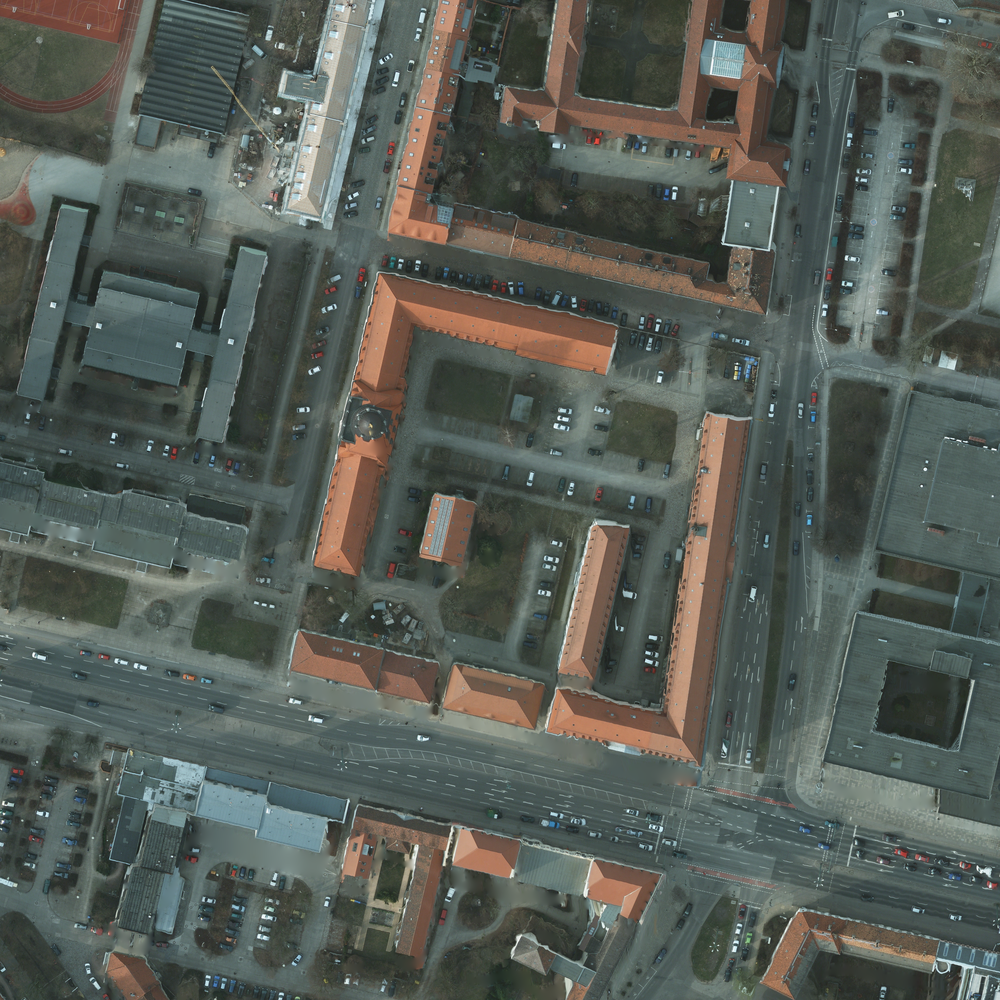
\includegraphics[scale=0.15]{input}
\caption{A overhead image with a resolution of 30 cm/pixel}
\end{figure}
\end{frame}


\begin{frame}
  \frametitle{\hfill Previous techniques}

  \begin{block}{Earlier methods}
    \begin{itemize}
    \item Sliding window techniques
    \item Aggregating pixels into super pixels before analysing
    \item Two stage segmentation networks
    \item Fast region-based convolutional neural networks (fast R-CNN)
    \end{itemize}
  \end{block}

\end{frame}



\begin{frame}
\frametitle{\hfill Two stage segmentation networks}
\begin{figure}[h!]
\centering
      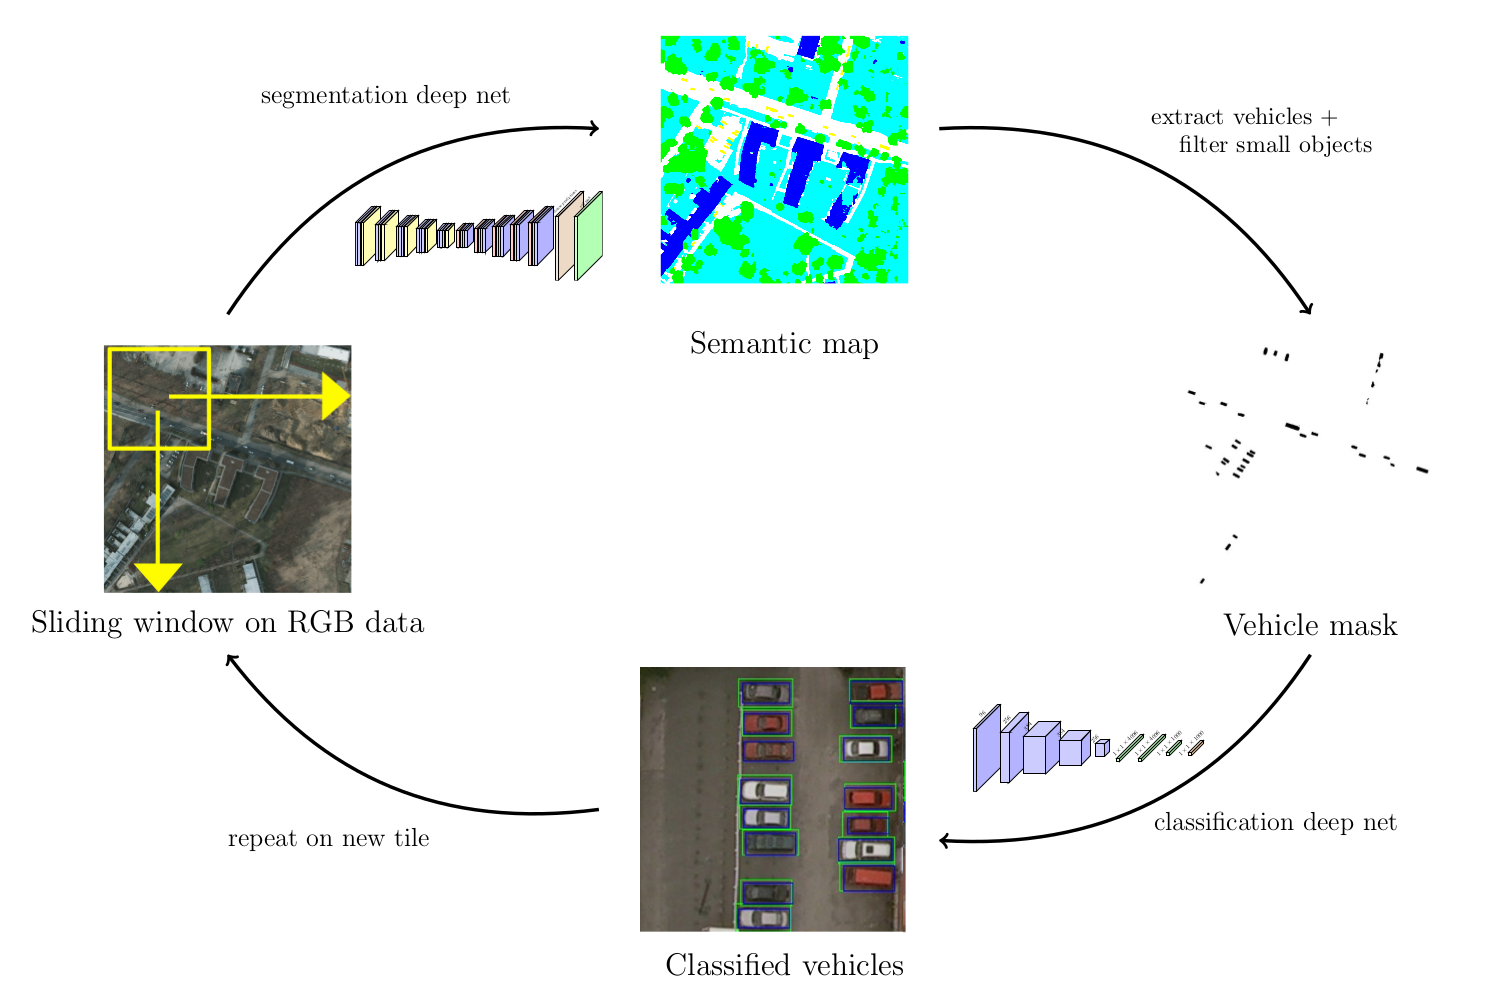
\includegraphics[scale=0.18]{SBD_net}
\caption{The Segment Before you Detect network structure} \label{fig:SBD}
\end{figure}
\end{frame}



\begin{frame}
  \frametitle{\hfill Fast R-CNN}
\begin{figure}[h!]
\centering
      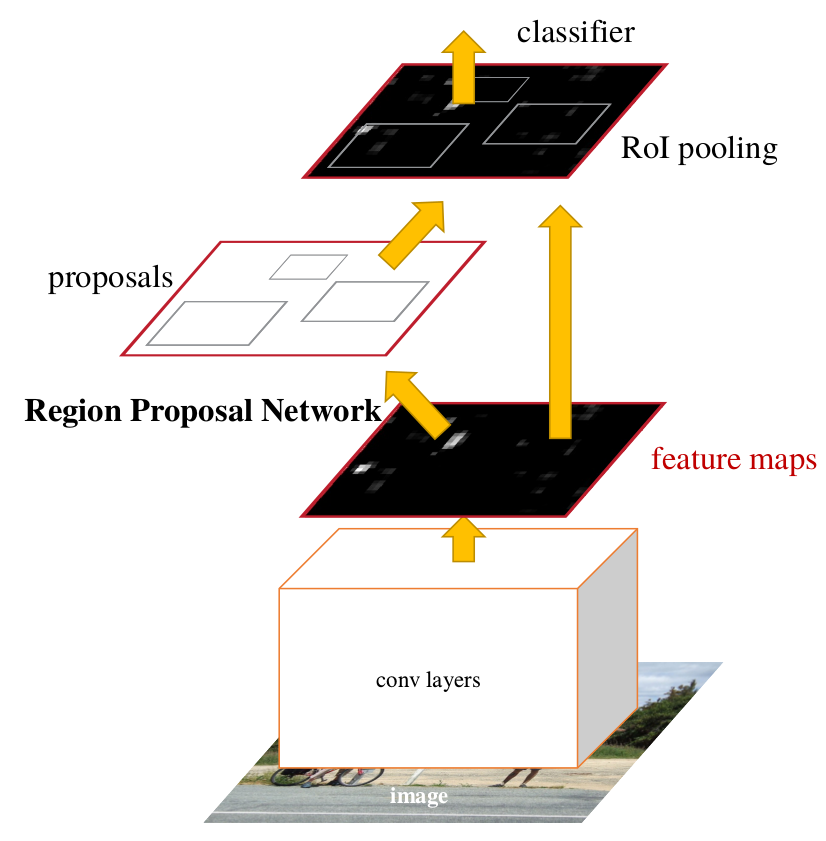
\includegraphics[scale=0.18]{r-cnn}
\caption{The two stage fast R-CNN} \label{fig:SBD}
\end{figure}
\end{frame}



\begin{frame}
  \frametitle{\hfill Previous techniques}
	  \begin{block}{Drawbacks}
    \begin{itemize}
    \item Segment Before you Detect is slow due complex structure with two deep networks
    \item Fast R-CNN can only predict some predefined ratios of bounding boxes which affects the precision
    \end{itemize}
  \end{block}
\end{frame}



\begin{frame}
  \frametitle{\hfill The goal}
	  \begin{block}{Extract vehicles directly from the segmentation map}
    \begin{itemize}
    \item Superior speed compared to Segment Before you Detect methods
    \item A more general approach compared to fast R-CNN since arbitrary size bounding boxes can be predicted
    \item The final network will be more simple considering only one stage is needed.
    \end{itemize}
  \end{block}
\end{frame}



\begin{frame}
  \frametitle{\hfill Proposed Model}
\begin{figure}[h!]
\centering
      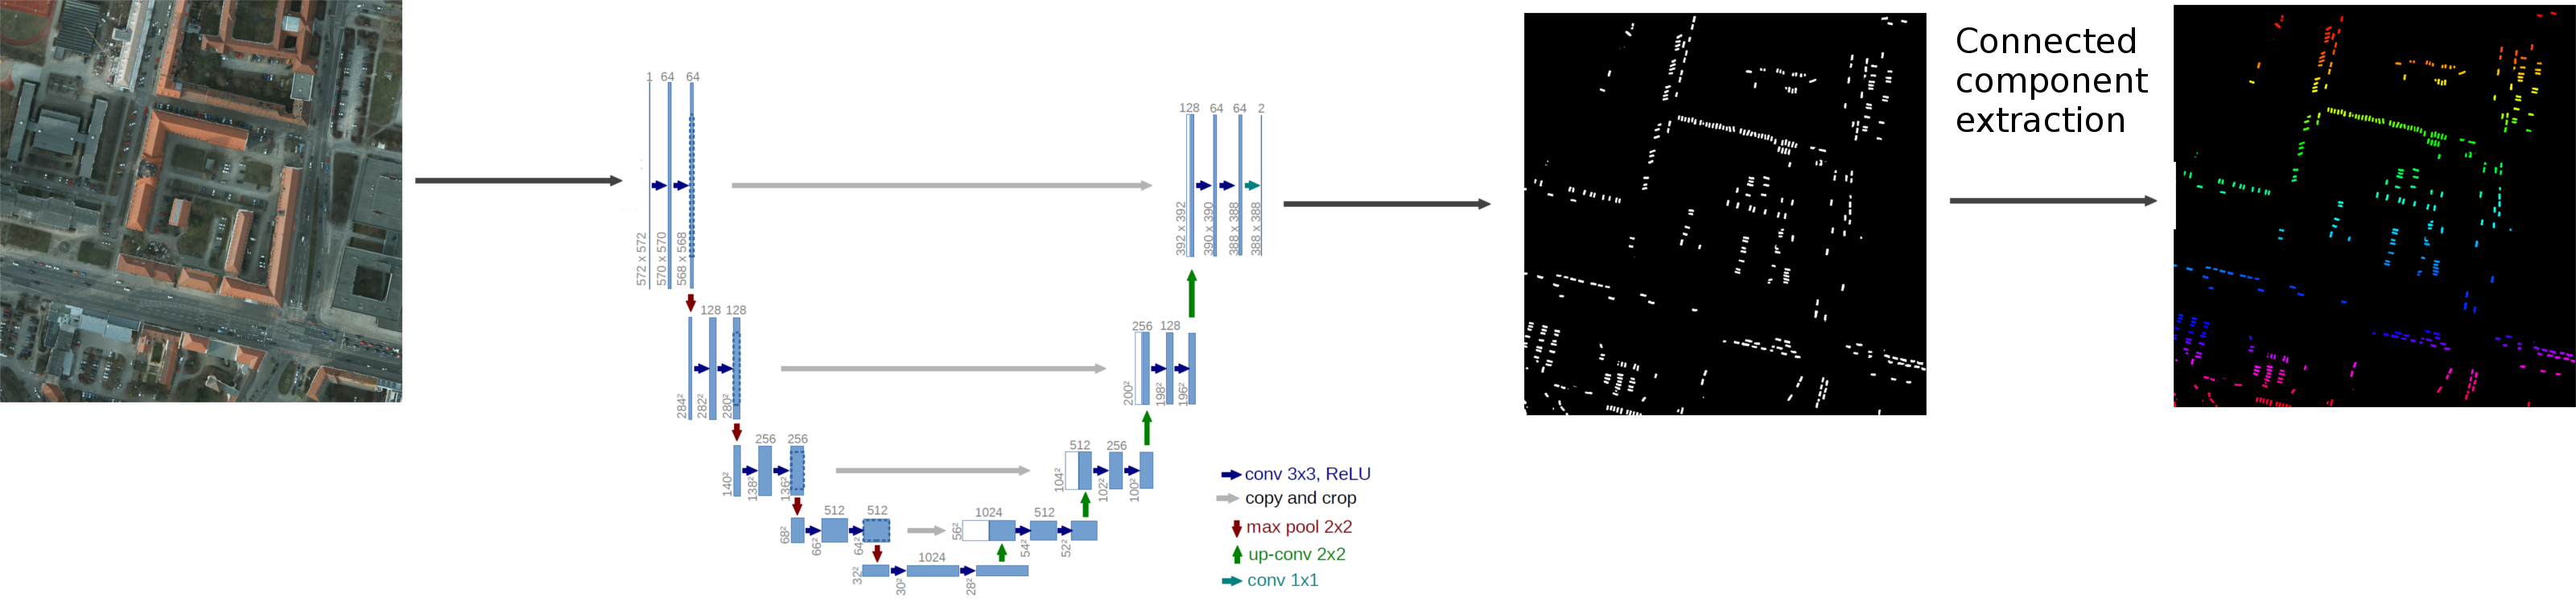
\includegraphics[scale=0.15]{net}
\caption{The architecture of the proposed model}
\end{figure}
\end{frame}




\begin{frame}
  \frametitle{\hfill The problem}
	  \begin{block}{The normal cross entropy loss does not enforce object separation sufficiently}
    \begin{itemize}
    \item Small separations between vehicles are likely to be overlooked
    \end{itemize}
  \end{block}
  \begin{block}{Find a loss function that enforces object separation}
    \begin{itemize}
    \item Adding an adversarial loss term
    \item Weighting the cross entropy loss based on vehicle separation
    \end{itemize}
  \end{block}
\end{frame}



\begin{frame}
  \frametitle{\hfill Adding an adversarial loss term}
\begin{figure}[h!]
\centering
      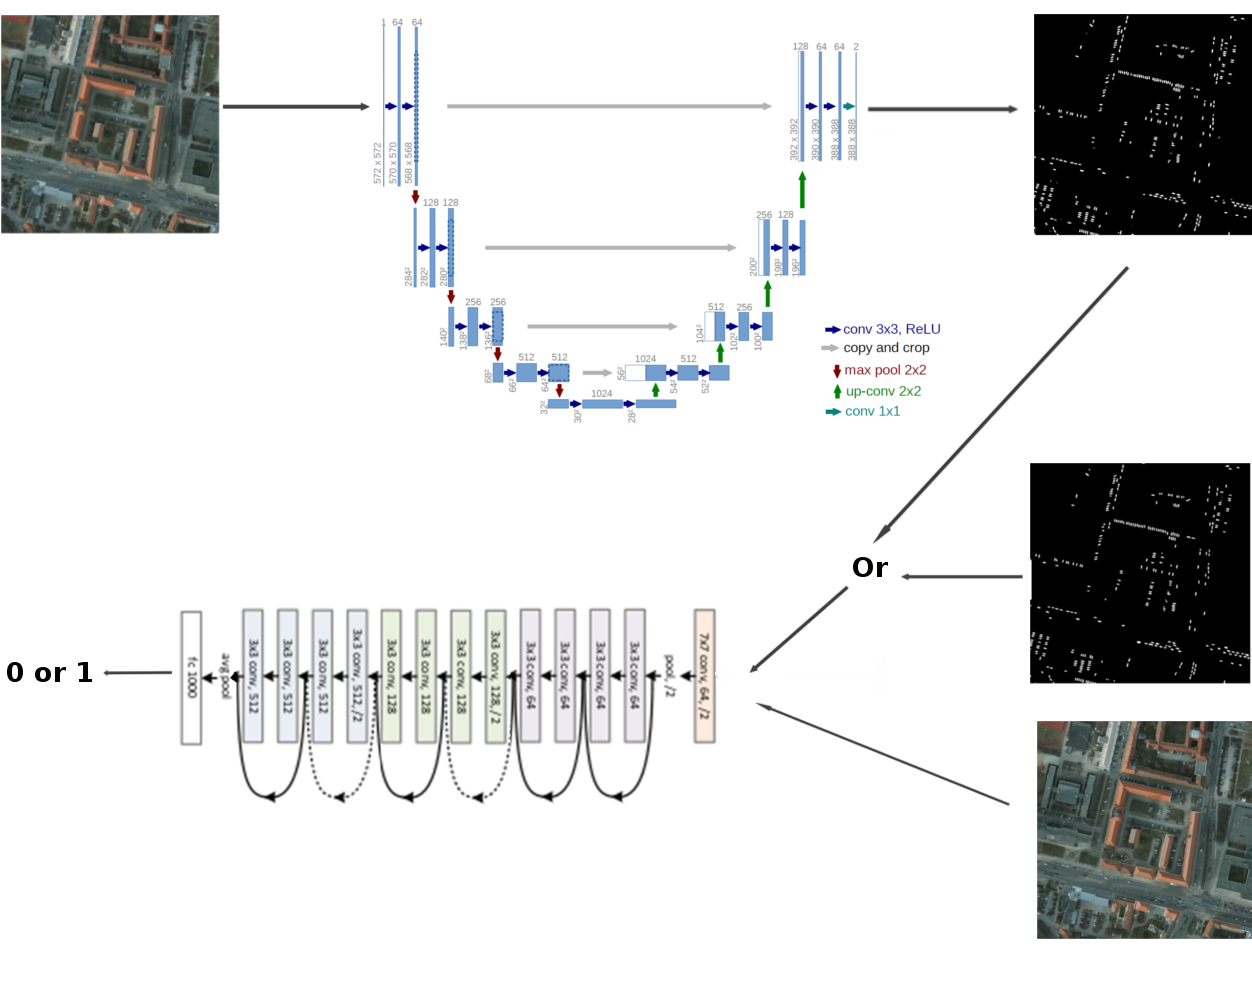
\includegraphics[scale=0.18]{gan}
\caption{The generative adversarial network architecture} \label{fig:SBD}
\end{figure}
\end{frame}




\begin{frame}
  \frametitle{\hfill Adding an adversarial loss term}
	  \begin{block}{Builds on a counterfeit game between the semantic and discriminating network}
	  \begin{equation*}
\ell_{bce}(\hat{y}, y)=-(y*ln(\hat{y})+(1-y)*ln(1-\hat{y}))
\end{equation*}
	  \begin{equation*}\label{eq:mce}
	\ell_{pxl}(\hat{y}, y) = - \sum_{x=1}^{H*W}y(x)*log(\hat{y}(x))
	\end{equation*}

\begin{equation*}
\Lagr(G) =\ell_{bce}(D(x,G(x)), 1) + \lambda\ell_{pxl}(G(x),y)
\end{equation*}
\begin{equation*}
\Lagr(D) =\ell_{bce}(D(x,G(x)), 0) + \ell_{bce}(D(x,y), 1)
\end{equation*}
  \end{block}
\end{frame}



\begin{frame}
  \frametitle{\hfill Weighting the cross entropy loss}
	  \begin{block}{Enforce the network to learn small separations between vehicles}
	  \begin{equation*}\label{eq:mce}
	\ell_{pxl}(\hat{y}, y) = - \sum_{x=0}^{H*W}\omega(x)*y(x)*log(\hat{y}(x))
	\end{equation*}

\begin{equation*}
\omega(x)=\omega_c+\omega_0*epx(\frac{(-d_1(x)-d_2(x))^{2}}{2\sigma^2})
\end{equation*}
\begin{equation*}
\omega_c=2\textit{, }\omega_0=10\textit{, }\sigma=3
\end{equation*}
  \end{block}
\end{frame}


\begin{frame}
  \frametitle{\hfill Weighting the cross entropy loss}
\begin{figure}[h!]
\centering
      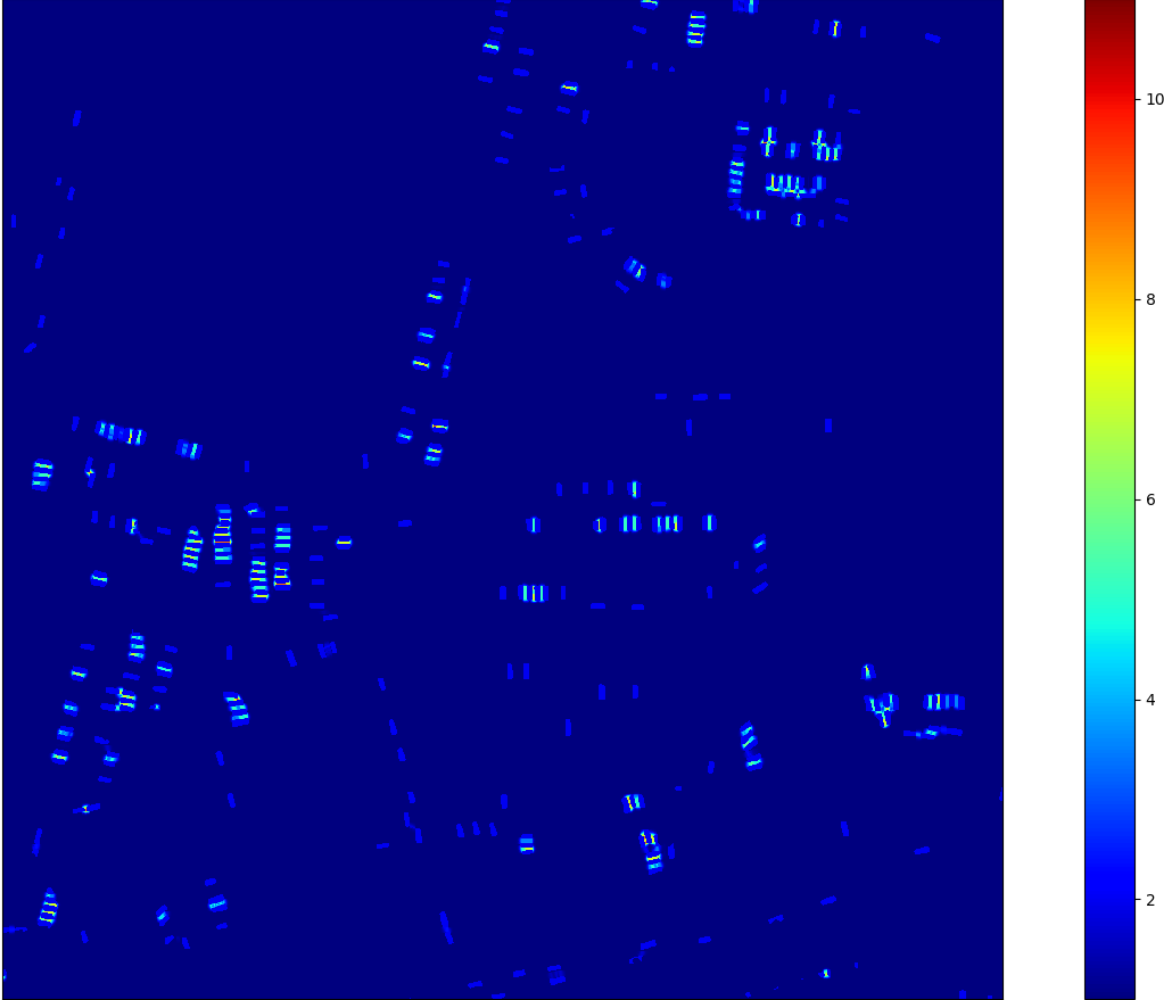
\includegraphics[scale=0.18]{weight_map_3}
\caption{The pixel wise weight map used to enforce seperations between vehicles} \label{fig:SBD}
\end{figure}
\end{frame}

\begin{frame}
  \frametitle{\hfill The datasets}
	  \begin{block}{The model will be evaluated on two datasets}
    \begin{itemize}
        \item The ISPRS Potsdam dataset
        \begin{itemize}
    \item A segmentation dataset
    \item 5 cm/pixel resolution
    \item $\approx$ 98 \% of all pixels belong to  the background class
    \item Images will be down sampled to 30 cm/pixel to match resolution of commercial satellite images.
    \item 24 images for training and validation, 14 for testing.
    \end{itemize}
    \item The Vedai dataset
    \begin{itemize}
    \item A vehicle detection dataset
    \item Vehicles are marked with bounding boxes
    \item 25 cm/pixel resolution
    \item Severe class imbalance $\approx$ 99.3 \% of all pixels belong to the background class
    \item 927 images for training, 100 for validation, 240 for testing.
    \end{itemize}
    \end{itemize}
  \end{block}
\end{frame}


\begin{frame}
  \frametitle{\hfill The Potsdam dataset}
\begin{figure}[H]
\minipage{0.40\textwidth}
  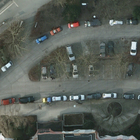
\includegraphics[width=\linewidth]{trees}
\endminipage\hfill
\minipage{0.40\textwidth}
  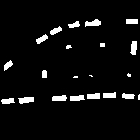
\includegraphics[width=\linewidth]{trees_label}
\endminipage\hfill
\caption{The left image shows the input image and the right image the ground truth segmentation}
\end{figure}
\end{frame}


\begin{frame}
  \frametitle{\hfill Evaluation metrics}
  A vehicle is defined as detected if the intersect over union of its predicted area and its ground truth area is greater than 0.5
	  \begin{equation*}\label{eq:mce}
	IoU = \frac{A_{pred}\cap A_{true}}{A_{pred} \cup A_{true}}>0.5
	\end{equation*}

\begin{equation*}
Precision=\frac{True\textit{ }positive}{True\textit{ }Positive+False\textit{ }poitive}
\end{equation*}
\begin{equation*}
Recall=\frac{True\textit{ }positive}{True\textit{ }Positive+False\textit{ }negative}
\end{equation*}
\begin{equation*}
F1\textit{ }score=\frac{2*Recall*Precision}{Recall+Precision}
\end{equation*}
\end{frame}



\begin{frame}
  \frametitle{\hfill Results: Adding a adversarial loss term}
\begin{figure}[H]
\minipage{0.32\textwidth}
  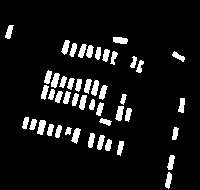
\includegraphics[width=\linewidth]{gan_vs_class/label_1}
\endminipage\hfill
\minipage{0.32\textwidth}
  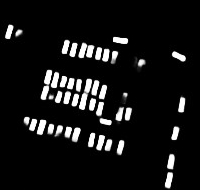
\includegraphics[width=\linewidth]{gan_vs_class/class_1}
\endminipage\hfill
\minipage{0.32\textwidth}%
  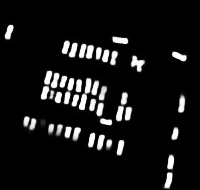
\includegraphics[width=\linewidth]{gan_vs_class/gan_1}
\endminipage
\caption{The the ground truth segmentation, the soft prediction without and with an adversarial loss}
\end{figure}
\end{frame}



\begin{frame}
  \frametitle{\hfill Results: Adding a adversarial loss term}
\begin{figure}[H]
\minipage{0.32\textwidth}
  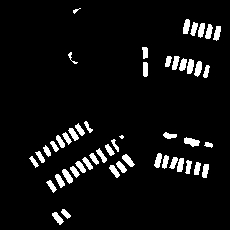
\includegraphics[width=\linewidth]{gan_vs_class/label_2}
\endminipage\hfill
\minipage{0.32\textwidth}
  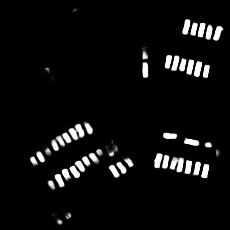
\includegraphics[width=\linewidth]{gan_vs_class/class_2}
\endminipage\hfill
\minipage{0.32\textwidth}%
  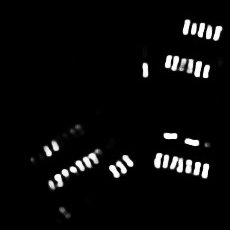
\includegraphics[width=\linewidth]{gan_vs_class/gan_2}
\endminipage
\caption{The the ground truth segmentation, the soft prediction without and with an adversarial loss}
\end{figure}
\end{frame}


\begin{frame}
  \frametitle{\hfill Results: Adding a adversarial loss term}
  The network with an adversarial loss was much more unstable, harder to train and did not increase the F1 pixel wise score on the validation dataset.
\begin{center}
\begin{figure}[H]
      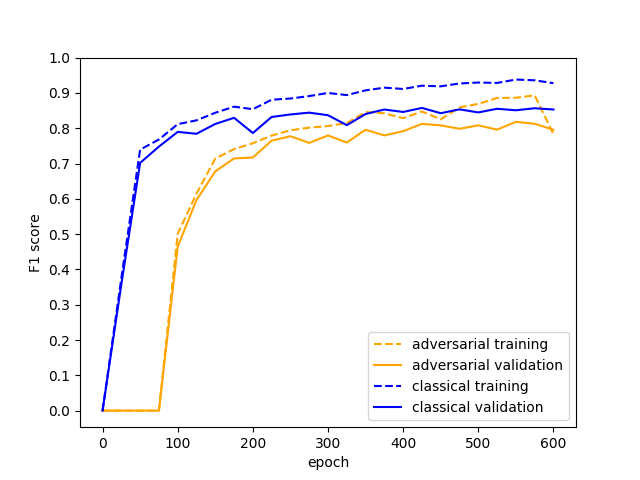
\includegraphics[scale=0.4]{classical_vs_adversarial}
  \caption{The F1 pixel wise score with and without an adversarial loss} \label{fig:gan_vs_class}
\end{figure}
\end{center}
\end{frame}


\begin{frame}
  \frametitle{\hfill Results: Weighting the loss function}
\begin{figure}[H]
\minipage{0.32\textwidth}
  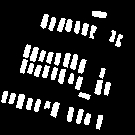
\includegraphics[width=\linewidth]{class_vs_w/label_1}
\endminipage\hfill
\minipage{0.32\textwidth}
  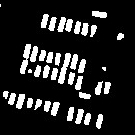
\includegraphics[width=\linewidth]{class_vs_w/un_weight_1}
\endminipage\hfill
\minipage{0.32\textwidth}%
  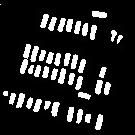
\includegraphics[width=\linewidth]{class_vs_w/weight_1}
\endminipage
\caption{The ground truth segmentation, the hard prediction with and without a weighted loss function}
\end{figure}
\end{frame}


\begin{frame}
  \frametitle{\hfill Results: Weighting the loss function}
\begin{figure}[H]
\minipage{0.32\textwidth}
  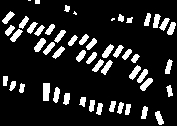
\includegraphics[width=\linewidth]{class_vs_w/label_2}
\endminipage\hfill
\minipage{0.32\textwidth}
  
\includegraphics[width=\linewidth]{class_vs_w/un_weight_2}
\endminipage\hfill
\minipage{0.32\textwidth}%
  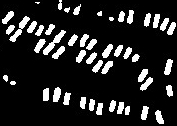
\includegraphics[width=\linewidth]{class_vs_w/weight_2}
\endminipage
\caption{The ground truth segmentation, the hard prediction with and without a weighted loss function}
\end{figure}
\end{frame}


\begin{frame}
  \frametitle{\hfill Results: Weighting the loss function}
  Weighting the loss function enforced better object separation while obtaining comparable pixel wise F1 score.
\begin{center}
\begin{figure}[H]
      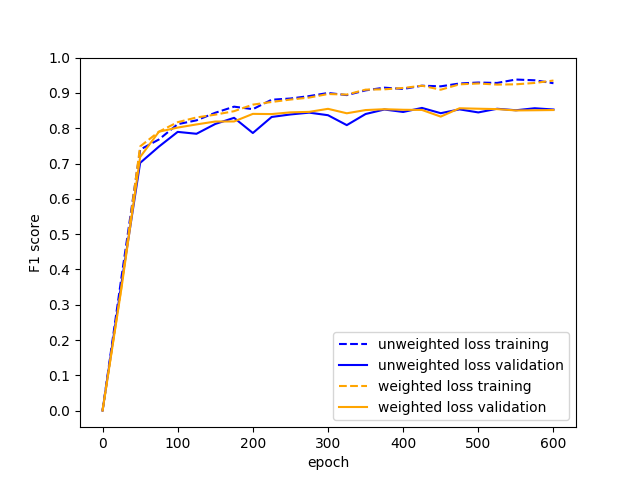
\includegraphics[scale=0.4]{class_vs_w}
  \caption{The F1 pixel wise score with and without loss weighting} \label{fig:gan_vs_class}
\end{figure}
\end{center}
\end{frame}


\begin{frame}
  \frametitle{\hfill Final results on the Potsdam dataset}
\begin{figure}[H]
\minipage{0.47\textwidth}
  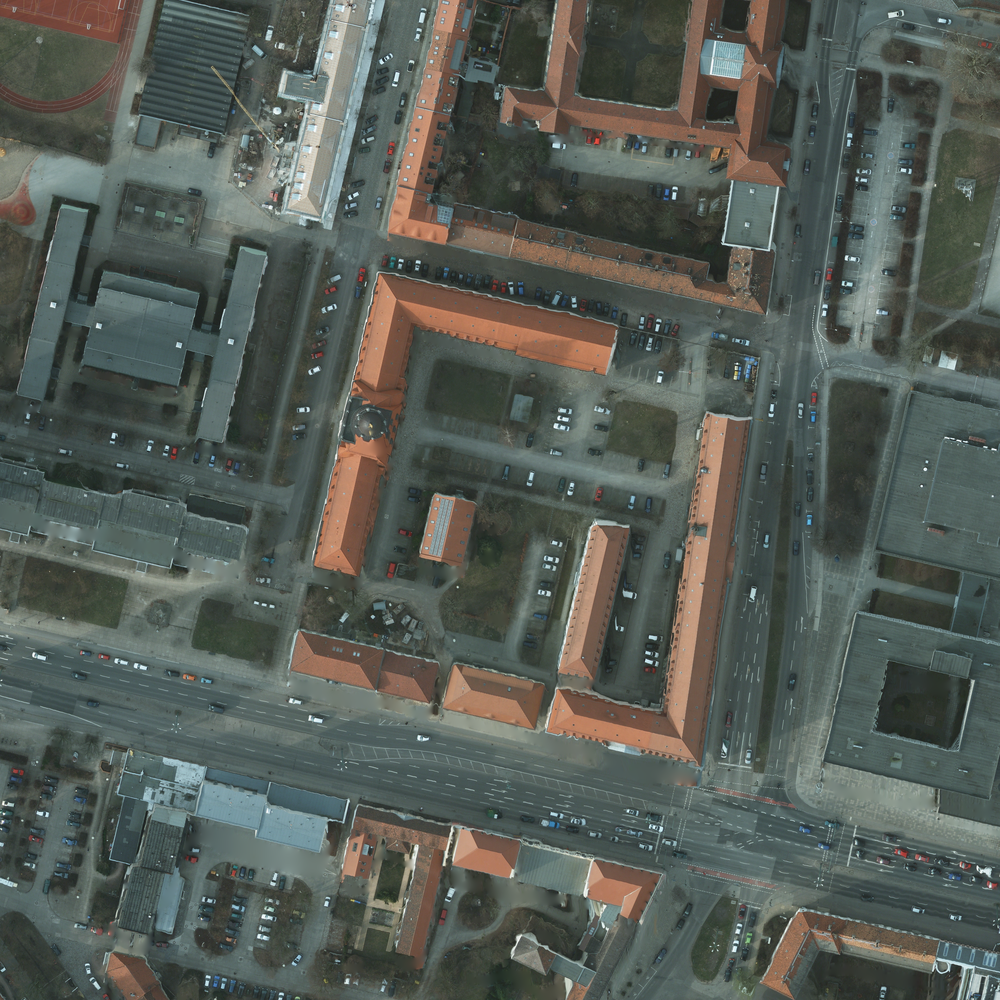
\includegraphics[width=\linewidth]{input}
\endminipage\hfill
\minipage{0.47\textwidth}
  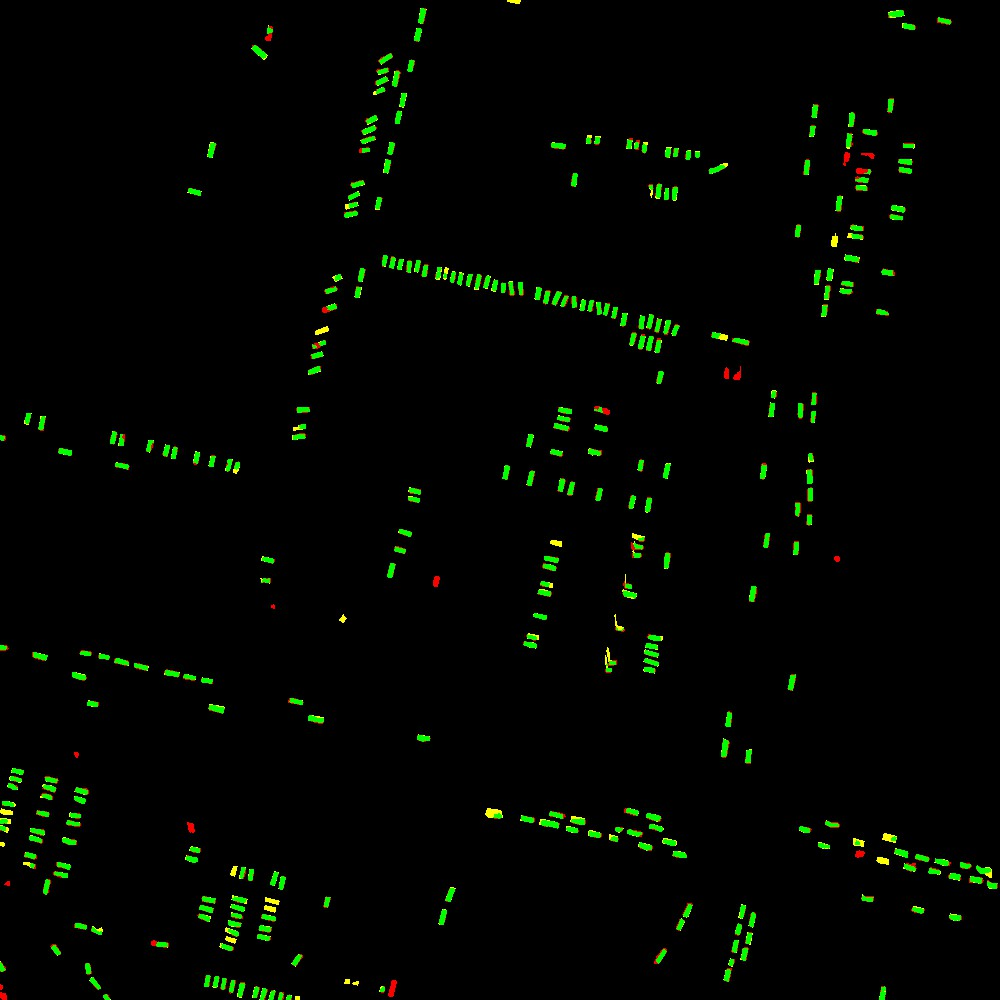
\includegraphics[width=\linewidth]{out}
\endminipage\hfill
\caption{The input and output segmentation. Green is true positives, yellow are false negatives and red are false positives.}
\end{figure}
\end{frame}


\begin{frame}
  \frametitle{\hfill Final results on the Potsdam dataset}
	  \begin{block}{Vehicle detection}
    \begin{itemize}
    \item The proposed model obtains a pixel wise F1 score 0.851
    \item The proposed model obtains a vehicle wise F1 score 0.811
    \item Mean evaluation time per image is 0.19 seconds = 2 seconds per square kilometre 
    \end{itemize}
  \end{block}
\end{frame}


\begin{frame}
  \frametitle{\hfill Final results on the Potsdam dataset}
	  \begin{block}{Counting cars}
    \begin{itemize}
    \item The connected components of the predicted segmentation and the ground truth segmentation were extracted and counted
    \item Mean prediction error of 1.67 \%
    \end{itemize}
    \begin{tabular}{|c c c c c c c|}
\hline
\textbf{Tile \#} & 2\_11  & 2\_12 & 7\_9 & 7\_10 & 7\_11 & 7\_12 \\
\hline
\textbf{Number of vehicles} & 107 & 123 & 304 & 250 & 346 & 346 \\
\textbf{Predicted number of vehicles} & 108 & 126 & 310 & 251 & 352 & 337 \\
\textbf{Prediction error in \%} &0.9 &  2.4 & 1.9 & 0.4 & 1.7 & 2.7\\
\hline
\end{tabular}
  \end{block}
\end{frame}



\begin{frame}
  \frametitle{\hfill Comparison with earlier work on Potsdam}
\captionof*{table}{}
\begin{tabular}{|c | c | c|}
\hline
\textbf{Model} & Proposed Model & SBD \\
\textbf{Resolution used} & \textbf{30 cm/pixel} & 12.5 cm/pixel\\
\textbf{Pixel wise F1 score} & 0.851 & \textbf{0.884}\\
\textbf{Vehicle wise F1 score} & \textbf{0.811} &  0.773\\
\textbf{Mean prediction error counting cars} & \textbf{1.67 \%} &  3.57 \%\\
\textbf{Evaluation time per image *} & \textbf{0.19 seconds} &  28.19 seconds\\
\hline
\end{tabular}\caption{Shows the comparison between the proposed model and the Segment before you Detect (SBD) model \parencite{audebert_usability_2016} on the Potsdam dataset. \textbf{*} The SBD model was evaluated on a Tesla K20 which can at maximum perform $3.52*10^{12}$ 32 bit floating point operations per second. The proposed model was evaluated on a Tesla K80 which can perform at maximum $8.74*10^{12}$ 32 bit floating point operations per second. Therefore the evaluation time on the SBD model was multiplied with $3.52/8.74\approx0.4027$ to make a fair comparison.}
\end{frame}


\begin{frame}
  \frametitle{\hfill Comparison with earlier work on Vedai}
  \captionof*{table}{}
\begin{tabular}{|c | c c|}
\hline
\textbf{Model} & \textbf{Detection time per image *}  & \textbf{Vehicle wise F1 score}\\
\hline
Faster R-CNN (Z\&F) & 0.1998 & 0.212\\
Faster R-CNN (VGG-16) & 0.2248 & 0.225\\
Fast R-CNN (VGG-16) & 3.1465 &  0.224\\
CCNN &0.2736 &  0.305\\
Proposed Model & \textbf{0.0616} & \textbf{0.542}\\
\hline
\end{tabular}
\caption{Shows the comparison between the proposed model and the Faster R-CNN (Z\&F), Faster R-CNN (VGG-16), Fast R-CNN (VGG-16) \cite{zeiler_visualizing_2014} and the Cascaded Convolutional Neural Networks (CCNN) \cite{zhong_robust_2017-1} on the Vedai dataset. \textbf{*} The other models were evaluated by \cite{zhong_robust_2017-1} on a Titan X which can at maximum perform $11*10^{12}$ 32 bit floating point operations per second. The proposed model was evaluated on a Tesla K80 which can perform at maximum $8.74*10^{12}$ 32 bit floating point operations per second. Therefore the evaluation time on the compared models were multiplied with $11/8.74\approx1.2586$ to make a fair comparison.}
\end{frame}


\begin{frame}
  \frametitle{\hfill Final conclusions}
	  \begin{block}{Proposed model characteristics}
    \begin{itemize}
    \item The proposed model has a computational time which is only a fraction of the SBD model while also obtaining higher vehicle wise F1 score and lower counting prediction error.
    \item The proposed model can use much lower resolution images which makes it a viable method for detecting and counting cars in satellite images.
    \item The proposed model outperforms the R-CNN models with a significant margin while also obtaining a slightly lower computational time.
    \item The proposed model only need a few images for training which means that  building new datasets for training is a low cost operation.
    \item The objects need to have a separation for connected component extraction to work. This can however be solved by introducing an ''artificial'' separation between touching objects.
    \end{itemize}
  \end{block}
\end{frame}


\begin{frame}
\printbibliography[heading=bibintoc]
\end{frame}
%\begin{frame}
%  \frametitle{\hfill The problem}
%
%  \begin{block}{Steps needed}
%    \begin{itemize}
%    \item Copy the following files:
%    \begin{itemize}
%    \item \texttt{examplepresentation.tex} (this file)
%    \item \texttt{beamerthemeKTH.sty}
%    \item \texttt{kthgraphics} (with all its contents)
%    \end{itemize}
%    \item Replace the contents in \texttt{examplepresentation.tex} with your own
%    \item Run \texttt{pdflatex} a couple of times
%    \item Present your slides using a PDF-viewer
%    \end{itemize}
%  \end{block}
%
%\end{frame}

\end{document}
